\documentclass{article}
\usepackage[brazil]{babel}
\usepackage[utf8]{inputenc}
\usepackage[T1]{fontenc}% optional T1 font encoding
\usepackage[%
    colorlinks=true,
    pdfborder={0 0 0},
    linkcolor=red
]{hyperref}
\usepackage[all]{hypcap}
\usepackage{amsmath}
\interdisplaylinepenalty=2500
\usepackage{graphicx}
\usepackage[cmintegrals]{newtxmath}
\usepackage{cite}
\usepackage{listings}
\usepackage{hyperref}
\usepackage{indentfirst}
\usepackage{siunitx}
\usepackage{textgreek}
\usepackage[portuguese,linesnumbered,ruled]{algorithm2e}
\usepackage{multirow}
\usepackage{anysize}

\begin{document}

    \title{Preparação do Exp. VI — Amplificador Operacional e Circuito Realimentado}
    \author{Bianca Yoshie Itiroko - 164923, Luiz Eduardo Cartolano - 183012, Seong Eun Kim - 177143 \\ EE534 - Turma Y - Grupo 2}
    \date{Novembro de 2018}

    \maketitle

    \section{Para o circuito da Figura \ref{fig:circ1}}
        \subsection{a) Relacione $V_a$ com $V_{in}$ e com $V_{pot}$}
            \begin{equation*}
                \frac{V_{pot} - V_{in}}{Z_1} = \frac{V_a - V_{pot}}{Z_2}
            \end{equation*}
            \begin{equation*}
                V_a = \frac{V_{pot} \cdot (Z_1 + Z_2) - V_{in} \cdot Z_2}{Z_1}
            \end{equation*}
            Como $Z_1=Z_2=1k\Omega$:
            \begin{equation*}
                V_a = 2 \cdot V_{pot} - V_{in}
            \end{equation*}
            
        \subsection{b) Relacione $V_c$ com $V_a$}
            \begin{equation*}
                \frac{V_a}{10K\Omega} = \frac{V_c - V_{c}}{100K\Omega}
            \end{equation*}
            \begin{equation*}
                10 \cdot V_a = V_{c} - V_a
            \end{equation*}
            Portanto:
            \begin{equation*}
                V_a = \frac{V_c}{11}
            \end{equation*}
            
         \subsection{c) Relacione $V_{out}$ com $V_c$}
            A relação existente entre $V_{out}$ e $V_c$ é a mesma existente entre um sinal de saída e um sinal de entrada de um \emph{circuito RC passa-alta} (como os vistos no primeiro laboratório), portanto:
            \begin{equation*}
                V_{out} = \frac{R}{\frac{1}{j\cdot\omega\cdot C} + R} \cdot V_c
            \end{equation*}
            Como $R = 8\Omega$ e $C = 220 \mu F$:
                \begin{equation*}
                    V_{out} = \frac{11 \cdot j \cdot \omega}{11 \cdot j \cdot \omega + 6250} \cdot V_{c}
                \end{equation*}
            
         \subsection{d) Determine qual é o laço de realimentação}
            O láco de realimentação presente no circuito da Figura \ref{fig:circ1} existe entre a saída do circuito \emph{push-pull} e a entrada negativa do segundo amplificador operacional (o que a entrada positiva está no topo).
            
         \subsection{e) Explique o funcionamento do circuito}
            A primeira parte do circuito da Figura \ref{fig:circ1}, que podemos considerar como encerrada na saída $V_A$, tem a função de regular o nível \emph{DC}, para isso, ela soma um valor ao sinal de entrada, o deslocando. Sua função é fazer com que o sinal de entrada do segundo amplificador operacional permita a operação de modo que seu sinal de saída seja capaz de polarizar o circuito \emph{push-pull} a fim de que ele funcione. 
            
            A realimentação, por sua vez, terá função parecida com a exercida pelos diodos no último experimento (vide \cite{}), ou seja, ela é responsável por garantir a polarização constante dos transistores e, por conseguinte, evitar a distorção do sinal de saída (observado em $V_{out}$).
           
    \section{Faça a simulação do circuito para $V_{in} = 100mV_{pp}$ a $1kHz$. Observe os sinais $V_a$, $V_b$ e $V_{out}$. Considere $C = 220\mu F$ e o alto-falante como uma carga $R_L = 8\Omega$. Ajuste o potenciômetro para que o circuito funcione adequadamente. }   
        A simulação pode ser observada em \cite{ref:simu}. Para que o circuito apresenta-se o comportamento esperado ajustou-se o potenciômetro de modo que ele tivesse $R_1 = 975\Omega$ e $R_2 = 24\Omega$. E que, por ele, circule uma corrente de, aproximadamente, $12 mA$.
            
    \nocite{*}
    \bibliographystyle{plain}
    \bibliography{references}

    \begin{figure}[!h]
        \centering
        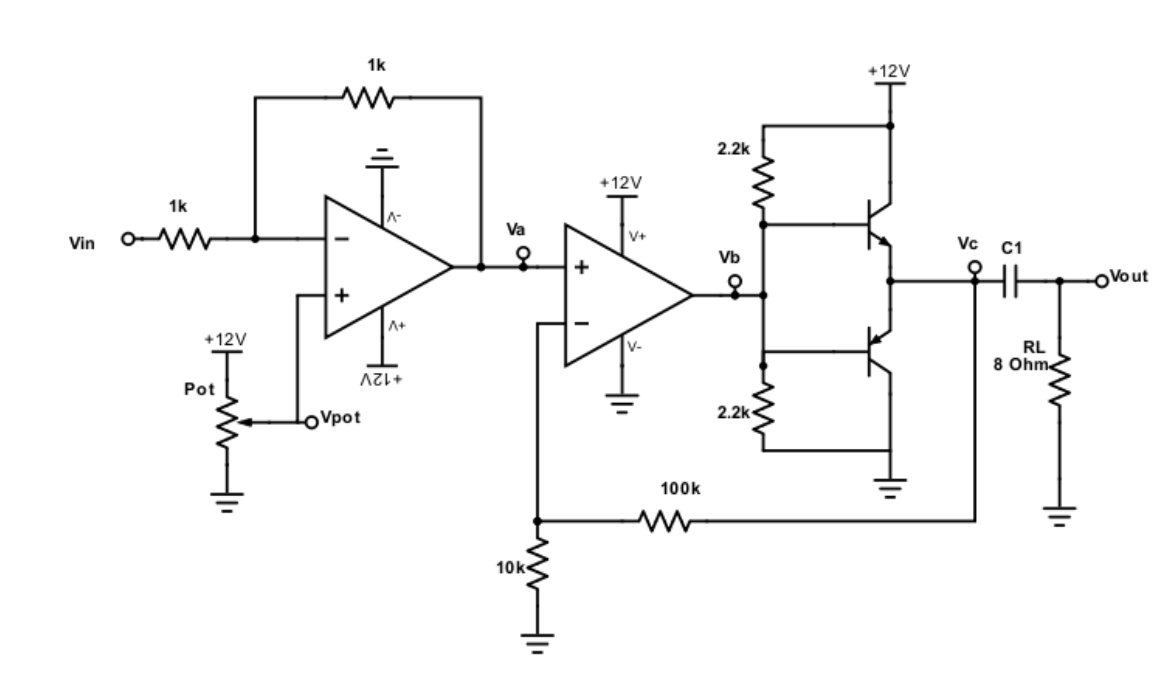
\includegraphics[height=9cm]{circ1.png}
        \caption{Circuito push-pull com alimentação não simétrica e realimentação.}
        \label{fig:circ1}
    \end{figure}
    
    

\end{document}

